\def\baselinestretch{0.91}

%%%%%%%%%%%%%%
%%% Appendix A
%%%%%%%%%%%%%%

\chapter{Acronyms}\label{Acronyms}


For clarity, we list many TAA
(Technical Acronyms and Abbreviations)
employed in our review. We do not include names of experiments and collaborations, up to some exceptions.
 

\begin{multicols}{2}
\begin{itemize}
\item[ADM] Asymmetric Dark Matter.
\item[AGN] Active Galactic Nucleus.
\item[AU] Astronomical Unit.
\item[BAO] Baryonic Acoustic Oscillations.
\item[BBN] Big Bang Nucleosynthesis.
\item[BH] Black Hole.
\item[BR] Branching Ratio.
\item[BSM] Beyond the SM.
\item[CC] Cosmological Constant.
\item[CDM] Cold Dark Matter.
\item[CHAMP] CHArged Massive Particle (of DM).
\item[CIB] Cosmic Infrared Background.
\item[CL] Confidence Level.
\item[CMB] Cosmic Microwave Background.
\item[CMSSM] Constrained Minimal Supersymmetric Standard Model.
\item[COB] Cosmic Optic Background.
\item[CP] Charge Conjugation times Parity.
\item[CPT] CP times Time reversal.
\item[CR] Cosmic Rays.
\item[DD] Direct Detection (of Dark Matter).
\item[DE] Dark Energy.
\item[DED] Dark Energy Domination.
\item[DFSZ] Dine-Fischler-Srednicki-Zhitnitskii axion.
\item[DIS] Deep Inelastic Scattering.
\item[DM] Dark Matter.
\item[DM$\nu$] Neutrinos from DM annihilations.
\item[EBL] Extragalactic Background Light.
\item[EFE] External Field Effect (in MOND).
\item[EFT] Effective Field Theory.
\item[dof] degree of freedom.
\item[FIMP] Freeze-In Massive Particles.
\item[FIMP] Feebly Interacting Massive Particles.
\item[FLRW] Friedmann-Lema\^itre-Robertson-Walker (equations). 
\item[FS] Free Streaming.
\item[GC] Galactic Center of the Milky Way.
\item[GCH] Galactic Center Halo (a `small' region around the GC).
\item[GH] Galactic Halo.
\item[GloC] Globular Cluster.
\item[GR] General Relativity.
\item[GRB] Gamma Ray Burst.
\item[GUT] Grand Unified Theory.
\item[GW] Gravitational Wave.
\item[HDM] Hot Dark Matter.
\item[HEP] High Energy Physics.
\item[HS] Haloscope.
\item[HST] Hubble Space Telescope.
\item[IACT] Imaging Atmospheric \v Cerenkov Telescope.
\item[IC] Inverse Compton.
\item[ICS] Inverse Compton Scattering.
\item[ID] Indirect Detection (of Dark Matter).
\item[IDM] Inert Doublet Model/Inert Higgs.
\item[IGM] InterGalactic Medium.
\item[IMBH] Intermediate Mass Black Hole.
\item[ISRF] InterStellar Radiation Field.
\item[JWST] James Webb Space Telescope.
\item[KSVZ] Kim-Shifman-Vainstein-Zakharov axion.
\item[$\Lambda$CDM] The standard cosmological model featuring a CC and CDM.
\item[$\Lambda$D] CC / DE Domination.
\item[LEP] the most recent $e\bar{e}$ collider at CERN.
\item[LHC] Large (or Last) Hadron Collider.
\item[LKP] Lightest Kaluza-Klein Particle.
\item[LSP] Lightest (Stable) SuperSymmetric Particle.
\item[LSS] Large Scale Structure.
\item[LSS] Last Scattering Surface.
\item[LSW] Light Shining through a Wall (experiment).
\item[MACHO] Massive Astrophysical Compact Halo Object.
\item[MB] Maxwell-Boltzmann distribution.
\item[MD] Matter Domination. 
\item[MDM] Minimal Dark Matter.
\item[MOND] MOdified Newtonian Dynamics.
\item[MSP] Milli-Second Pulsar.
\item[MSSM] Minimal Supersymmetric Standard Model.
\item[MReq] Matter-Radiation equality. 
\item[MW] Milky Way.
\item[NFW] Navarro, Frenk and White DM density distribution.
\item[NLSP] Next-to-Lightest SuperSymmetric Particle.
\item[NRO] Non Relativistic Operator.
\item[NRO] Non Renormalizable Operator.
\item[NS/ns] Neutron Star.
\item[PBH] Primordial Black Hole.
\item[PDF] Parton Distribution Function.
\item[PDF] Probability Distribution Function.
\item[PIMP] Planckian Interacting Massive Particle.
\item[pNGB] pseudo-Nambu-Goldstone boson.
\item[PTA] Pulsar Timing Array.
\item[QCD] Quantum Chromo Dynamics.
\item[QED] Quantum Electro Dynamics.
\item[QFT] (Relativistic) Quantum Field Theory.
\item[QSO] Quasi-Stellar Object (Quasar).
\item[RD] Radiation Domination.
\item[SHM] Standard Halo Model.
\item[SIDM] Self-Interacting Dark Matter.
\item[SIMP] Strongly Interacting Massive Particle.
\item[SIGW] Scalar Induced Gravitational Waves.
\item[SM] Standard Model of particles.
\item[SMBH] Super-Massive Black Hole.
\item[SN] Supernova.
\item[SNR] Supernova Remnant.
\item[SSM] Standard Solar Model.
\item[SUSY] SUperSYmmetry.
\item[TeVeS] Tensor-Vector-Scalar theory.
\item[vev] vacuum expectation value.
\item[VIB] Virtual Internal Bremsstrahlung.
\item[WD/wd] White Dwarf.
\item[WDM] Warm Dark Matter.
\item[WIMP] Weakly Interacting Massive Particle.
\item[WMAP] Wilkinson Microwave Anisotropy Probe.
\end{itemize}
\end{multicols}

\def\baselinestretch{1}

%%%%%%%%%%%%%%
%%% Appendix B
%%%%%%%%%%%%%%

\chapter{Basic notations and conventions}\label{Conventions}

\begin{multicols}{2}
\begin{itemize}
\item[$a_0$] $=1/\alpha m_e\approx 1/3.7\keV$, Bohr radius.
\item[$\alpha$] $=e^2/4\pi\approx 1/137.036$, fine-structure constant.
\item[$\alpha_{\rm s}$] $=g_{\rm s}^2/4\pi$, strong coupling constant.
\item[$\alpha_2$] $=g_2^2/4\pi$, weak $\SU(2)_L$ coupling constant.
\item[$\alpha_Y$] $=g_Y^2/4\pi$, hypercharge coupling constant.
\item[$d\eta:$] conformal time, $d\eta=dt/a$.
\item[$\eta$:]  baryon-to-photon number density ratio, $\eta =  n_{\rm b}/n_\gamma$.
\item[$\eta$:]  slow roll parameter in inflation.
\item[$\epsilon$:]  slow roll parameter in inflation.
\item[$\epsilon$:]  kinetic mixing.
\item[$f_{a}$:] axion decay constant.
\item[$g_{\rm s}$:] strong gauge coupling.
\item[$g_2$:] weak $\SU(2)_L$ gauge coupling.
\item[$g_Y$:] hypercharge gauge coupling.
\item[$h$:] Higgs boson 
\item[$h$:]  the scaling factor for Hubble expansion rate defined through $H_0 = h\times 100\km/{\rm sec\cdot Mpc}$.
\item[$H$:] Higgs doublet. 
\item[$H$:] Hubble expansion rate.
\item[$H_0$:] present-day Hubble expansion rate.
\item[$K$:] kinetic energy.
\item[$\Lambda_{\rm QCD}$] $\approx 300\MeV$, non-perturbative QCD scale.
\item[$M$:] DM mass.
\item[$M_h$] $\approx 125\GeV$, Higgs boson mass.
\item[$m_N$] $ \approx 0.939\GeV$, nucleon mass. We mostly work in the isospin limit $m_N=m_p=m_n$.
\item[$m_a$:] axion mass.
\item[$m_n$:] neutron mass.
\item[$m_p$:] proton mass.
\item[$M_{\odot}$]$\approx 1.988\,10^{30}\,\text{kg}=1.115\,10^{57}\,\text{GeV}$, solar mass.
\item[$M_{\oplus}$] $\approx 5.972\,10^{24}\,\text{kg}=3.350\,10^{51}\,\text{GeV}$, Earth mass. 
\item[$M_{\rm Pl}$] $\approx 1.2 \,10^{19}\GeV$, Planck mass.
\item[$\bar{M}_{\rm Pl}$:] reduced Planck mass, $\bar{M}_{\rm Pl}^2 = {M}_{\rm Pl}^2/8\pi $.
\item[$M_t$] $\approx 171\GeV$, top quark mass.
\item[$n_{\rm b}$:]  number density of baryons.
\item[$n_{\gamma}$:]  number density of photons.
\item[$\Omega_{\rm b}$:] cosmological abundance of normal baryonic matter, see eq.~\eqref{eq:Omegai}.
\item[$\Omega_{\rm DM}$:] cosmological abundance of dark matter, see eq.s~\eqref{eq:OmegaDMh2}, \eqref{eq:Omegai}.
\item[$\wp$]: pressure.
\item[Pf]: Pfaffian.
 \item[$s_{\rm W}$:] $\sin\theta_{\rm W}$, sinus of the weak angle.
\item[$\tau$:] DM lifetime.
\item[$T_{\rm eq}$] $\approx 0.8\eV$ temperature at matter-radiation equality.
\item[$T_{\rm U}$] $\approx 13.7~{\rm Gyr}$, the age of the Universe.
\item[$T_0$] $\approx 2.726$\,K, present CMB temperature.
\item[$v$] $\approx 174\GeV$, the Higgs vacuum expectation value.
\item[$Y$:] hypercharge, normalized such that the electric charge is $Q=T_3+Y$.
\end{itemize}
\end{multicols}

%%%%%%%%%%%%%%
%%% Appendix C
%%%%%%%%%%%%%%

\chapter{Cosmology}
\label{app:Cosmology}


In this appendix we collect some of the main results from big-bang cosmology, which are used throughout the main text.

\section{Big bang expansion}

The expanding Universe, assumed to be homogenous and isotropic (in agreement with observations, at least on large enough scales) is described by the translation and rotation invariant Friedmann-Lema\^itre-Robertson-Walker (FLRW) metric 
\beq 
ds^2 = - dt^2 + a^2(t)\left[ \frac{dr^2}{1-k\, r^2} +r^2 \, d\theta^2 +r^2 \sin^2\theta \, d\phi^2 \right] \stackrel{({\rm if} \ k = 0)}{=} - dt^2 + a^2(t) [dx^2 + dy^2 +dz^2],
\eeq
where $a(t)$ is the scale factor and $k = 0, \pm1$ is a constant that describes the global geometry ($k=0$ for flat, $k=+1$ for closed, i.e.,~the geometry of a sphere, and $k=-1$ for open geometry, i.e.,~the geometry of a hyperbolic surface). The fact that $a$ depends on time encodes the expansion. In the usual convention, $a(t)$ is dimension-less and is normalized in such a way that it equals unity today, $a( t = T_U) = a_0 = 1$. Conventionally, one also defines the cosmological redshift $z$ as $1+z = 1/a$, so that today $z_0 = 0$.

\medskip

The matter-energy content of the Universe is modeled as a generic fluid, whose stress-energy tensor is constrained by the homogeneity and isotropy to have the form
\beq 
T^\mu_\nu = \diag(\rho,p,p,p),
\eeq
where $\rho$ is the energy density and $p$ the pressure. 
In such a Universe, Einstein's equations of general relativity,
$R_{\mu\nu} - {\cal R}g_{\mu\nu}/2= 8\pi G~ T_{\mu\nu} $,
specialize to the Friedmann equations
\beq
\label{eq:FRWeq}
\displaystyle H^2 = \frac{8\pi G}{3}\rho - \frac{k}{a^2}, \qquad
\displaystyle \frac{\ddot{a}}{a} = -\frac{4 \pi G}{3} (\rho+3p),
\eeq
where the dot operator (~$\dot{}$~) denotes the derivative with respect to time $t$. Here, $H\equiv \dot a/a$ is the {\em Hubble expansion rate}. Note that $H$ is not constant in time.  In general, it varies as $H\propto 1/t$ in the phases of interest (see eq.~\eqref{eq:aandHinMDRD} below). Its present value is the so called {\em Hubble `constant'}, $H=H_0$, where
\beq 
H_0 = h \frac{100\,{\rm km}}{{\rm sec}\cdot\,{\rm Mpc}} = 
\frac{h}{9.78~10^9\,{\rm yr}} = 2.1 \, h~ 10^{-33}\eV,\qquad
h \approx 0.7,
\eeq
with parsec equal to 1\,pc$=3.26$\,lyr. 

Some of the equations simplify, if one uses instead of time $t$, the {\em conformal time}
$\eta$, defined as the comoving distance traveled by light (we always set $c=1$)
\beq
d\eta \equiv  dt/a(t)= da/Ha^2.
\eeq

\medskip

It is fun to note that the first Friedmann equation in \eqref{eq:FRWeq} could have been derived already 
by Newton (up to the `Jeans swindle'), centuries before Einstein, Friedmann, Robertson and Walker. 
Indeed, modeling the Universe as a sphere with radius $a(t)$ composed by a constant density $\rho(t)$, the Newtonian gravity
predicts that it evolves according to  
\beq \ddot{a}= - \frac{G M(r<a)}{a^2}=
-\frac{4\pi G\rho(t)}{3} a .\eeq
Taking into account that for matter one has $\rho(t)\propto 1/a^3(t)$
this equation can be integrated,  obtaining the usual conservation of energy
$$ \frac{d}{dt}\left[ \frac{1}{2}\dot{a}^2-\frac{4\pi}{3}G\rho a^2\right]=0,$$
from which eq.~(\ref{eq:FRWeq}) follows.

The constant $k$ in \eqref{eq:FRWeq} plays the role of an energy constant. The critical case of `zero energy',  $k=0$,
corresponds to a density that is equal to the `critical density',
\beq 
\label{eq:rhocrit}
\rho =  \rho_{\rm cr}\equiv 3H^2/8\pi G, 
\eeq
and describes a Universe that expands ``for free'' (the double of zero energy is zero energy).
This is the case predicted by the inflationary cosmology in general relativity, and is compatible with the present observations of the actual Universe.

\medskip


\section{Matter-energy content}\label{app:matterenergy}

Many components of the Universe are described by a simple equation of state 
\beq  \label{eq:p=wrho}
p=w\rho\qquad\hbox{with $w$ a constant.}
\eeq
The relativistic conservation law for the energy momentum tensor, $T^{\mu\nu}{}_{;\nu}=0$,
 gives the first law of thermodynamics:
\beq dU =-p\,dV,
\qquad 
U = \rho V.
\eeq
The explicit solution is $\rho \propto a^{-3(1+w)}$.
The relevant special cases are:
\begin{itemize}

\item $w=0$ describes {\em non-relativistic matter} (`dust'), $p_m=0$ and $\rho_m \propto 1/a^3$;

\item $w=1/3$ describes {\em relativistic particles} (`radiation'): $p_r=\rho_r/3$ and $\rho_r \propto 1/a^4$;

\item $w=-1$ describes {\em vacuum energy}: $p_V=-\rho_V$ and $\rho_V \propto {\rm const,}$, with $a$.

\end{itemize}
The actual Universe is composed from a sum of different components: matter, radiation and dark energy. The dark energy contribution is at present observationally consistent with it being just  the vacuum energy, and it might thus be described simply by a nonzero cosmological constant $\Lambda$, without any dynamics. 
The present energy densities of these components are conventionally expressed in terms of ratios with respect to the critical density
\beq
\label{eq:Omegai}
 \Omega_i = \rho_i/\rho_{\rm cr} .
 \eeq
They are measured to be~\cite{PDG,Planckresults} 
\beq
\label{eq:Omegas}
 \Omega_\Lambda \simeq 68.5\%,\qquad
 \Omega_m \simeq 4.9\%+26.4\%,\qquad
 \Omega_r \simeq 0.0054\%+0.0037\%, \qquad
 \sum_i \Omega_i \simeq 1 .
\eeq
The matter contribution has two components:
normal baryonic matter ($\Omega_{\rm b}\simeq 4.8\%$) and the unknown Dark Matter ($\Omega_{\rm DM}\simeq 25.8\%$), the subject of this review.
Radiation is also made out of two components: photons (0.0054\%, as per the energy density of a blackbody with temperature $T_{\rm CMB} = 2.7255$ K) and neutrinos, here considered massless (0.0037\%, as they contribute as 3.046 effective fermionic species, each with a temperature $(4/11)^{4/3} \, T_{\rm CMB}$).
Since the three components $\Omega_{\Lambda}, \Omega_m,$ and $\Omega_r$, evolve differently with $a$, their relative weights in the composition of the Universe changes with time.
From fig.~\ref{fig:Omegas}, we can see that matter started dominating the Universe at $a>a_{\rm eq} = \Omega_r/\Omega_m\approx 1/3400$,
i.e., at $t_{\rm eq}\approx 60\,{\rm kyr}$ (Matter-Radiation equality, MReq). 



\begin{figure}[t]
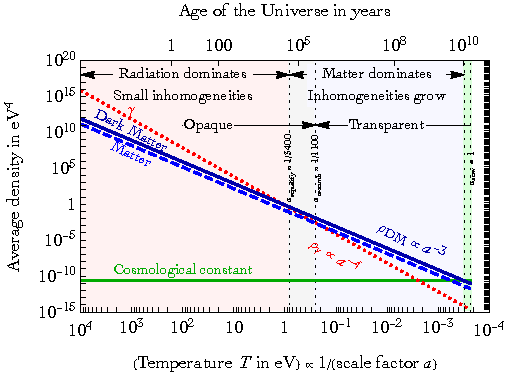
\includegraphics[width=0.5\textwidth]{figs/rhoCosmoReview} \quad
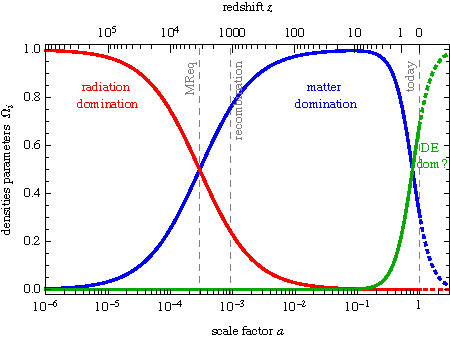
\includegraphics[width=0.46\textwidth]{figs/Omegas_in_cosmology}
\caption[Time evolution of the components of the Universe]{\em  \label{fig:Omegas} 
{\bfseries Evolution of the components of the (flat) Universe} as a function of time or  temperature (left), and a simplified version showing the dominant component as a function of the scale factor $a$ or the redshift $z$ (right). }
\end{figure}


\medskip

The age of the Universe is given by
\beq T_U  = \int_0^1 \frac{da}{a \, H} = 
\frac{1}{H_0}
\int_0^1 \frac{da}{a\sqrt{\Omega_\Lambda + \Omega_m/a^3 + \Omega_r/a^4}}=
\frac{1}{H_0}\times\left\{\begin{array}{ll}
1/2 & \hbox{if $\Omega_r = 1$,}\\
2/3 & \hbox{if $\Omega_m=1$,}\\
0.96 & \hbox{our Universe.}
\end{array} \right.
\eeq
In general, one can solve numerically the Friedmann equation (\ref{eq:FRWeq})
\beq 
\label{eq:FRWexplicit}
\frac{\dot a}{a} = H = H_0 \sqrt{\frac{\rho}{\rho_0}} = H_0 \sqrt{\Omega_\Lambda + \frac{\Omega_m}{a^3} + \frac{\Omega_r}{a^4}} \ . \eeq
Simple analytic results hold for the epochs in which either matter (MD) or radiation (RD) dominated the total energy density,
\beq 
\label{eq:aandHinMDRD}
a(t) = \left\{\begin{array}{l}
(2 t H_0 )^{1/2}    \\
(3t H_0 /2)^{2/3}   
\end{array}\right.   \qquad
H(t) = \left\{\begin{array}{ll}
  1/(2t) & \hbox{during RD at $a\ll a_{\rm eq}$,}  \\
  2/(3t) & \hbox{during MD at $1\gg a\gg a_{\rm eq}$.} 
\end{array}\right.
\eeq






\section{Particles in thermal equilibrium}
\label{sec:app:particles:thermal}

A gas of relativistic particles at temperature $T$ has energy $E\sim T$,
wavelength $\lambda \sim 1/T$, and consequently number density $n_{\rm eq}$ and
energy density $\rho_{\rm eq}$ approximatively given by
\beq  n_{\rm eq}\sim T^3,\qquad \rho_{\rm eq}\sim T^4.\eeq
For non relativistic particles, $T\ll m$, one instead has $E\simeq m$ 
such that $\rho_{\rm eq} = m n_{\rm eq}$ and
both densities get suppressed by a Boltzmann factor $e^{-m/T}$
(unless there is a conserved quantum number that prevents such suppression, e.g., the baryon number
in the case of baryonic matter).

\smallskip

The precise formul\ae{} for the thermal densities of a gas of particles with mass $m$ and $g$ degrees of freedom are:
\begin{eqnarray}
n_{\rm eq}(T) &=&   g\int\frac{d^3p}{(2\pi)^3} f_{\rm eq}
=\frac{g}{2\pi^2}\int_m^\infty  f_{\rm eq} E  p \, dE,
\\
\rho_{\rm eq}(T)&=&g\int\frac{d^3p}{(2\pi)^3} E f_{\rm eq}= 
\frac{g}{2\pi^2}\int_m^\infty  f_{\rm eq} E^2 p\,dE,
 \\
p_{\rm eq}(T) &=&   g\int\frac{d^3p}{(2\pi)^3}\frac{p^2}{3E} f_{\rm eq}
=\frac{g}{6\pi^2}\int_m^\infty  f_{\rm eq} p^{3} \, dE,
\end{eqnarray}
where $f_{\rm eq} = 1/(e^{E/T}+c)$ is
the Fermi-Dirac distribution for fermions ($c=+1$) or the 
Bose-Einstein distribution for bosons ($c=-1$).
A simple useful approximation is the Boltzmann limit $c=0$.
\begin{itemize}
\item[$\triangleright$] In the ultra-relativistic limit, $T\gg m$, the integrals can be performed easily, with the
explicit results given by
\beq \label{eq:relativisticquantities}
n_{\rm eq}(T\gg m)=\frac{g}{\pi^2} T^3\times \left\{
\begin{array}{ll}
3\zeta(3)/4&\hbox{$c=+1$,}\\
1&         \hbox{$c=0$,}\\
\zeta(3)  &\hbox{$c=-1$,}
\end{array}\right.
\eeq
\beq 
\rho_{\rm eq}(T\gg m)=\frac{g}{\pi^2} T^4\times \left\{
\begin{array}{ll}
7\pi^4/240&\hbox{$c=+1$,}\\
3&         \hbox{$c=0$,}\\
\pi^4/30  &\hbox{$c=-1$,}
\end{array}\right.\eeq
and $p_{\rm eq}=\rho_{\rm eq}/ 3$. 
The total energy density in relativistic species, which can have different temperatures, is then given by
\beq
\rho_{\rm R}(T) = \frac{\pi^2}{30} g_\rho(T) \, T^4, \qquad {\rm with} \quad g_\rho(T) = \sum_{m\ll T}  g_{\rm b} \left( \frac{T_{\rm b}}{T}\right)^4+ \frac{7}{8} \sum_{m\ll T} g_{\rm f} \left(\frac{T_{\rm f}}{T}\right)^4,
\eeq
where the two sums run over bosons and fermions, respectively. 

\item[$\triangleright$]
In the non-relativistic limit, $T\ll m$, all the distributions reduce to the Boltzmann result,
\beq \label{eq:nnonrel}
n_{\rm eq}(T\ll m) = g(mT/2\pi)^{3/2} e^{-m/T}, \qquad
p_{\rm eq} \ll \rho_{\rm eq} \simeq m n_{\rm eq}.
\eeq

\item[$\triangleright$] For generic $T$, one can obtain analytic expressions by
approximating the quantum distributions with a Boltzmann distribution 
\beq n_{\rm eq} \approx \frac{g m^2 T}{2\pi^2}{\rm K}_2\left(\frac{m}{T}\right),
\qquad \rho_{\rm eq} \approx  \frac{g m^2 T}{2\pi^2}\left[m \,{\rm K}_1\left(\frac{m}{T}\right)+
3T\, {\rm K}_2\left(\frac{m}{T}\right)\right],
\eeq
where $K_{1,2}(x)$ denote the modified Bessel functions of the second kind.
\end{itemize}


\smallskip


\begin{figure}[t]
$$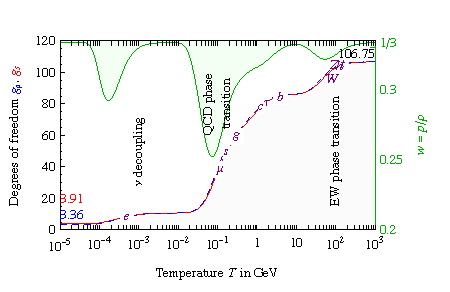
\includegraphics[width=0.7\textwidth]{figs/dofSMw}$$
\caption[Degrees of freedom in the SM]{\em  \label{fig:dofSM} 
Degrees of freedom of the SM $g_{\rm s}(T)$ (red) and $g_\rho(T)$ (blue dashed), increasing up to $106.75$ as function of the temperature $T$.
The green curve (with values on the right axis) shows the approximate value of $w=p/\rho$
(see~\cite{TQCD} for lattice computations).
}
\end{figure}



Since the Universe cannot exchange the heat with any ``outside'' system,  its evolution
in the thermal equilibrium conserves the entropy, $S=sV$,
where $V$ is the volume, and
\beq  \label{eq:sentropy}
s = \frac{\rho+p}{T} \equiv \frac{2\pi^2}{45}g_{s}(T) \, T^3, \qquad \hbox{is the entropy density.}
\eeq
Up to factors of order one, $s$ is essentially the total number density of particles, $n_{\rm eq}$.
Conservation of $S$ implies that the temperature $T$ decreases during expansion as $T\propto1/a$,
up to the decrease in the effective number of (entropy density) degrees of freedom, $g_{s}$. The latter takes place whenever the various SM particles become non relativistic and can no longer be produced by thermal processes in the plasma.
The entropy is dominated by the ultra-relativistic particles. Summing over all the relativistic degrees of freedom one thus has \beq 
g_{s} =  \sum_{m\ll T} g_{\rm b} \left(\frac{T_{\rm b}}{T}\right)^3+ \frac{7}{8} \sum_{m\ll T} g_{\rm f} \left( \frac{T_{\rm f}}{T} \right)^3,
\eeq
where $g_{\rm b,f}$ give the internal number of degrees of freedom (spin or any other internal quantum numbers) for each species of bosons and fermions. 
At 
high temperatures, all the SM fermions and bosons are in a thermal equilibrium and consequently have the
same temperature $T$: the value of $g_{\rm s}(T)$ in the SM is shown in fig.\fig{dofSM}. 
The effective number of degrees of freedom relevant for energy density, $g_\rho$, is defined analogously, but with $(T_{\rm b,f}/T)^4$ temperature ratios.
At $T\gg M_t$, such that all SM particles are ultra-relativistic, one has
$g_{s}=\frac{7}{8}2\cdot 3\cdot 15+2(1+3+8)+2\cdot 2=106.75$,
slightly lower than 118, the total number of SM degrees of freedom. This then slowly drops when different species of SM particles become non-relativistic.
For $T\sim \Lambda_{\rm QCD}$ the calculation of $g_{\rm s}$ is more complicated, see~\cite{TQCD} for details.
After neutrino decoupling, at $T\ll m_e$, the Universe contains
photons and neutrinos with different temperatures,
$T_\nu = T_\gamma (4/11)^{1/3}$.
Measuring the entropy in units of the photon temperature,
one has $g_{s} = 2 + \frac{7}{8} 2\cdot 3\frac{4}{11}=\frac{43}{11} \simeq 3.91$.

Additional light degrees of freedom that could be present in plasma are usually expressed in terms of the corresponding change of the effective number of neutrinos, $\Delta N_{\rm eff}$. \index{Effective number of neutrinos}
The SM value of $N_{\rm eff}^{\rm SM}$ is defined via the low temperature ratio of the neutrino energy, $\rho_\nu$, to the photon energy density, $\rho_\gamma$, 
\beq
\frac{\rho_\nu}{\rho_\gamma}\Big|_{T/m_e\to0} = \frac{7}{8} \Big(\frac{4}{11}\Big)^{4/3} N_{\rm eff}^{\rm SM}, 
\eeq
and is $N_{\rm eff}^{\rm SM}=3.044$ (it differs from 3 due to subleading effects such as the remaining small energy transport from photon plasma to the neutrino sector). The contribution of any new relativistic degrees of freedom to the energy density of plasma can then be parametrized similarly via 
\beq
\label{eq:DeltaNeff}
\frac{\rho_{\rm light~NP}}{\rho_\gamma}\Big|_{T/m_e\to0} = \frac{7}{8} \Big(\frac{4}{11}\Big)^{4/3} \Delta N_{\rm eff}. 
\eeq
Current cosmological bounds require $\Delta N_{\rm eff}\lesssim 0.3$.

\section{Particles out of thermal equilibrium}
If the system is in a thermal equilibrium, the description of its physical properties is rather simples since everything is dictated by the temperature $T$, and possibly by
the values of conserved quantum numbers such as the baryon number. 

However, during the cosmological evolution particles may go out of
thermal equilibrium. This is a potentially important effect for DM, since it can results in a relic abundance of DM. 
The criterion for the out of equilibrium dynamics can be succinctly stated as: {\em a particle is in thermal equilibrium, if $\Gamma \gg H$,
i.e.,\ if its interaction rate $\Gamma \sim n \sigma$ is faster than the rate of expansion, $H \sim T^2/M_{\rm Pl}$}.
The cross section $\sigma$ is determined by particle physics, where the interactions can be split into two broad categories:
\begin{itemize}
\item {\bf Renormalizable interactions}, whose strength is controlled by 
dimension-less couplings $g$.  Then
$\sigma \sim g^{2 -  4}/T^2$ and $\Gamma \sim g^{2 - 4} T$\
where the powers of $2$ and $4$ are, respectively, valid for $1\to 2$ and $2\to 2$ scatterings.
Since $H$ drops quadratically with smaller $T$, these interactions become {\em fast} (relative to $H$) at late times, when the temperature falls below
$T \circa{<} g^{2 - 4} M_{\rm Pl}$.  
For example, the electromagnetic, weak, and strong interactions have couplings
$e,g_2,g_3\sim 1$, and are in thermal equilibrium  for temperatures below $T \sim 10^{17}\GeV$.
The Yukawa interactions of charged SM particles span 5 orders of magnitude. The smallest one is the electron Yukawa coupling
$\lambda_e \sim 10^{-6}$. The interactions mediated by it enter in thermal equilibrium at $T\sim \TeV$ (this is of mainly academic interest since other interactions, namely the exchanges of gauge bosons already keep electrons and other SM particles in thermal equilibrium).

\item {\bf Non-renormalizable interactions}, whose strength is suppressed by powers of high scale, for instance, for dimension 6 interactions the dimensionful couplings are $\sim1/M^2$.
Then, for dimensional reasons, one has $\sigma\sim T^2/M^4$, $\Gamma \sim T^5/M^4$, so that such interactions become {\em slow} at late times $T\circa{<} M (M/M_{\rm Pl})^{1/3}$.
For example,  weak interactions at $T\ll M_{W,Z}$ are suppressed by $M\approx v$
and decouple at $T \sim\hbox{few MeV}$.
Electromagnetic interactions of electrons at $T\ll m_e$ are described by $M\approx m_e$,
allowing for photon decoupling
as $\Gamma \propto T^3 \sigma_{\rm T}\sim T^3/m_e^2$, where $\sigma_T$ is the Thomson cross section (although the formation of neutral hydrogen occurs earlier).



\end{itemize}
Particles that fall out of thermal equilibrium, i.e., particles with negligible interactions are easily described:
their wavelength expands with universe, such that $p \propto 1/a$.  Then:
\begin{itemize}
\item {\bf For relativistic particles} (such as neutrinos) this means $E=p\propto 1/a$: they maintain a
thermal distribution with $T\propto 1/a$, just as if they had remained in thermal equilibrium.\footnote{Note, however, that the temperature of the thermal plasma and the decoupled particles need not be the same. The temperature evolution for thermal plasma does not always follow $T\propto 1/a$ since the number of degrees $g_{\rm s}(T)$ may change as the plasma cools.}
\item
{\bf For non-relativistic particles} (such as possibly DM) this means that $E = p^2/2m \propto 1/a^2$:
they cool faster than particles in thermal equilibrium.
\end{itemize}
In summary:
$$\begin{array}{c|cc} 
& \hbox{massless},~ T\gg m & \hbox{massive},~ T\ll m\\ \hline
\hbox{interacting with the plasma} & T \propto 1/a& T \propto 1/a\\
\hbox{non-interacting with the plasma} & T \propto 1/a& T \propto 1/a^2
\end{array}$$


For example, electrons become non relativistic at $T\sim m_e$, at which point the neutrinos have already decoupled. 
Neutrinos remain relativistic for a long time, but are non-relativistic at present (at least the two species that are required to be massive by the neutrino oscillation measurements). 
The kinetic energy of DM particles after decoupling tends to be red-shifted away.


\section{Boltzmann equations}\label{Boltzmann}\index{Boltzmann equation}
Many important computations in cosmology are performed through the use of  Boltzmann equations. Below, we review this useful tool. 


In the absence of interactions the number of particles in a comoving volume $V$ remains constant.
Boltzmann equations then encode the effects of different interactions.
Let us study, e.g.,\ how the decays, $1\leftrightarrow 2+3$, and the inverse decays, $2+3\to1$,
affect the number of particles of species `1', given by the number density $n_1$ in volume $V$,
\begin{eqnarray}
\label{eq:Boltz1} \frac{d}{dt}(n_1 V) &=&V \int d\vec{p}_1\int d\vec{p}_2\int d\vec{p}_3\,
(2\pi)^4 \delta^4(p_1-p_2-p_3)\times\\
&&\times\nonumber [-|\mathscr{A}_{1\to 23}|^2 f_1(1\pm f_2)(1\pm f_3) + |\mathscr{A}_{23\to 1}|^2(1\pm f_1) f_2 f_3],
\end{eqnarray}
where $d\vec{p}_i = \sum d^3p_i/2E_i(2\pi)^3$ is the relativistic phase space of particle $i$
summed over the $g_i$ degrees of freedom (polarizations and multiplet components);
$|\mathscr{A}_{1\to 23}|^2$ and $|\mathscr{A}_{23\to 1}|^2$
are the squared transition amplitudes;
$f_i$ are the energy 
distributions of the various particles, where the plus (negative) signs in $(1\pm f_i)$ factors apply for $i$ particle that is a boson (fermion).
For simplicity we
assume that CP violation can be neglected, so that the decay and the inverse
decay process have a common amplitude $\mathscr{A}$.


In principle, one should study the evolution of all $f_i$ in order to obtain the total number densities 
$ n_i = \sum \int f_i~d^3p/(2\pi)^3$.
In practice, the elastic scatterings (i.e.,\ the interactions that do not change the number of particles and their species)
are typically fast enough that they maintain {\em kinetic equilibrium},
so that the full Boltzmann equations for $f$ are solved by 
$f(p) = f_{\rm eq}(p){n}/{n_{\rm eq}}$ where 
  $ \displaystyle  f_{\rm eq} = [e^{E/T}\pm 1]^{-1}$ are the thermal equilibrium Bose-Einstein and Fermi-Dirac distributions.
In this limit, each particle species is simply characterized by its total
abundance $n$,
that can be varied only by  inelastic processes.

  
  The factors $1\pm f_i$ in eq.\eq{Boltz1} take into account Pauli-blocking (for fermions) and stimulated emission (for bosons).
Since the average particle energy is $\langle E\rangle \sim 3T$ one can within $10\%$ accuracy set $1\pm f \approx 1$, one thus approximate $f_{\rm eq}$
with the Boltzmann distribution
$f_{\rm eq}\approx e^{-E/T}$.
This approximation then leads to significant simplifications in the results.



When the inelastic processes are also sufficiently fast to maintain {\em
chemical equilibrium},
the total number $n_{\rm eq}$ 
of particles with mass $M$ at temperature $T$ are given by
\beq\label{eq:neq}
n_{\rm eq}=g\!\int {d^3p~f _{\rm eq}\over(2\pi \hbar)^3}=\frac{gM^2T}{2\pi^2}
{\rm K}_2\biggr(\frac{M}{T}\biggr) = \left\{\begin{array}{ll}
{gT^3}/{\pi^2}, & T\gg M,\\
g(MT/2\pi)^{3/2}e^{-M/T}, & T\ll M,
\end{array}
\right.
\eeq
where $g$ is the number of spin, gauge, etc, degrees of freedom.
The factor $\hbar=h/2\pi$ has been explicitly shown to clarify the physical origin of the 
$2\pi$ in the denominator.


The Boltzmann equation for $n_1$ then simplifies to
\begin{eqnarray} \frac{1}{V}\frac{d}{dt}(n_1 V) &=& \int d\vec{p}_1\int d\vec{p}_2\int d\vec{p}_3\,
(2\pi)^4 \delta^4(p_1-p_2-p_3)\times\\
\nonumber &&\times  |\mathscr{A}|^2\left[- \frac{n_1}{n_1^{\rm eq}}
e^{-E_1/T} + \frac{n_2}{n_2^{\rm eq}}
\frac{n_3}{n_3^{\rm eq}}e^{-E_2/T}e^{-E_3/T}\right].
\end{eqnarray}
One can recognize that the integrals over final-state momenta reconstruct the decay rate $\Gamma_1$,
and that the integral over $d^3p_1/E_1$ averages it over the thermal distribution of initial state particles. The factor $1/E_1$ corresponds to the Lorentz dilatation of the lifetime.
The final result is therefore,
\beq\label{eq:Boltz2} \frac{1}{V}\frac{d}{dt}(n_1 V)
= \langle \Gamma_1 \rangle  n_1^{\rm eq}\left[ \frac{n_1}{n_1^{\rm eq}}- \frac{n_2}{n_2^{\rm eq}}
 \frac{n_3}{n_3^{\rm eq}}\right],
\eeq
where $\langle \Gamma_1\rangle$ is the thermal average of the Lorentz-dilatated decay width 
\beq
\Gamma_1(E_1) =\frac{1}{2E_1} \int d\vec{p}_2\, d\vec{p}_3 (2\pi)^4\delta^4(p_1-p_2-p_3) |\mathscr{A}|^2.
\eeq
 If $\langle \Gamma_1\rangle \gg H$, then the l.h.s. is much smaller than $ \langle \Gamma_1 \rangle  n_1^{\rm eq}$ and thus  the term in square brackets in eq.\eq{Boltz2} is forced to be vanishingly small.
 This just means that there are inelastic  interactions much faster than the expansion rate, which are able to enforce the chemical equilibrium,
giving  ${n} = {n}_{\rm eq}$.


Let us apply this to a concrete example, the $N_1\to LH$ decays in leptogenesis.  The $2,3=L,H$ particles have fast gauge interactions.
 Therefore we do not have to write and solve Boltzmann equations for $L,H$, because
 we already know their solution: $L,H$ are kept in chemical thermal equilibrium.
 We only need to insert this result in the Boltzmann equation for $N_1$, which then simplifies to
\beq 
\dot{n}_1 +3H n_1 = \langle\Gamma_1\rangle (n_1 - n_1^{\rm eq}),
\eeq
having used $\dot{V}/V =3H=-\dot s/s$.


In the numerical evaluations in computer codes one prefers to avoid very large or very small numbers. To achieve this 
it is convenient to reabsorb the $3H$ term, which accounts for the dilution due to the overall
expansion of the universe, by normalizing the number density $n$ to
the entropy density $s$.
Therefore, we study the evolution of  $Y = n/s$,
as function of $z=m_N/T$,
in place of time $t$.
Here, $H\, dt = d\ln R = d\ln z$, since during the adiabatic
expansion $sV$ is 
constant, i.e.,\ $V\propto 1/T^3$.
Expressed in terms of $Y(z)$ variables, the general form of the Boltzmann equations is
 \beq
 \label{eq:genericBoltz}  
sHz\frac{dY_1}{dz} = \sum
 \Delta_{1}\cdot
 \gamma_{\rm eq}(12\cdots \leftrightarrow 34\cdots)\left[
 \frac{Y_1}{Y_1^{\rm eq}}\frac{Y_2}{Y_2^{\rm eq}}\cdots-
 \frac{Y_3}{Y_3^{\rm eq}}\frac{Y_4}{Y_4^{\rm eq}}\cdots\right],
 \eeq
where the sum runs over all the processes that change the number of
`1' particles by $\Delta_1$ units (e.g.,\ $\Delta_1 = -1$ for the $1\to 23$ decay, while
$\Delta_1 = -2$ for the $11\to 23$ scatterings, etc.). The quantity  $\gamma_{\rm eq}$ is the 
space-time density of interactions (i.e.\ the number of interactions per unit volume and unit time) in thermal equilibrium for the various processes.

The direct and inverse processes 
have the same reaction densities, as long as
CP-violating effects can be neglected.
The explicit expressions for 1-body and 2-body processes are then, as follows:
\begin{itemize}
\item For a {\bf decay} and for its inverse process one gets the previous result,
\beq \gamma_{\rm eq}(1\,\to \,23) = S_f \sum_{\rm all}
\int d\vec{p}_1 \, f_1^{\rm eq}   \int  d\vec{p}_2\,d\vec{p}_3  
\, (2\pi)^4\delta^4(p_1-p_2-p_3) |\mathscr{A}|^2  = \gamma_{\rm eq}(23\,{\to} \,1),
\eeq
where the sum runs over all the final-state and initial-state indices 
(polarisations, components of gauge multiplets, etc), and
$S_f=1/n_f!$ is a symmetry factor, which differes from one, if the final state contains $n_f$ identical particles.
The thermal average of the decay rate can be analytically computed in terms of Bessel functions,
\beq\label{eq:gammaD}
 \gamma_{\rm eq}(1\to 23\cdots)=\gamma_{\rm eq}(23\cdots\to 1)= n^{\rm eq}_1
{\mbox{K}_1(z)\over\mbox{K}_2(z)}\,\Gamma(1\to 23\cdots) \eeq
with ${\mbox{K}_1(z)/\mbox{K}_2(z)}\simeq  1$ in the non-relativistic limit $z\gg 1$.

\item
For a {\bf 2-body scattering process}
\beq \label{eq:gamma2gen}
\gamma_{\rm eq}(12\,{\leftrightarrow}\,34) = 
S_i S_f\sum_{\rm all}
\int d\vec{p}_1\, d\vec{p}_2 \, f_1^{\rm eq}  f_2^{\rm eq}  \int  d\vec{p}_3\,d\vec{p}_4
\, (2\pi)^4\delta^4(p_1+p_2-p_3-p_4) |\mathscr{A}|^2, 
\eeq
where 
$$S_i=\left\{\begin{array}{ll}
1 & \hbox{if particles $1$ and $2$ are different},\\
1/2 & \hbox{if particles 1 and 2 are identical},
\end{array}\right.$$
is an initial-state symmetry factor analogous to $S_f$.
One can perform analytically almost all of the integrals, and obtain
\beq 
\label{eq:gamma2}
 \gamma_{\rm eq}(12\to 34\cdots)= 
{T\over 64\pi^4}\int_{s_{\rm min}}^{\infty}
ds~\sqrt{s}~  \hat{\sigma}(s)\  
\mbox{K}_1\!\left(\frac{\sqrt{s}}{T}\right), 
\eeq
where $s = (p_1+p_2)^2$ and $t= (p_1 - p_3)^2$ are the usual kinematical variables and
the dimension-less `reduced cross section' $\hat\sigma$ is defined as
\beq \hat \sigma = S_i S_f\sum_{\rm all}\int_{t_{\rm min}}^{t_{\rm max}} dt \frac{|\mathscr{A}|^2}{8\pi s}.\eeq
The sum is over the initial {\em and} the final state  indices.
\end{itemize}
One can express $\hat \sigma$ in terms of the usual cross section
\beq
 \hat \sigma=\sigma\times 2s S_ig_1 g_2 \lambda, 
\eeq
where $\sigma$ is summed over the final state, but {\em averaged} over the initial state indices, 
\beq
 \sigma  = \frac{S_f}{2E_1 2E_2 v}\sum_{\rm final} \int  d\vec{p}_3\,d\vec{p}_4
\, (2\pi)^4\delta^4(p_1+p_2-p_3-p_4)  \langle |\mathscr{A}|^2\rangle_{\rm initial}
=S_f\sum_{\rm final}  \int dt\frac{\langle   |\mathscr{A}|^2  \rangle_{\rm initial}}{16\pi s^2 \lambda}
.\eeq
The denominator,  $E_1 E_2 v =[(p_1\cdot p_2)^2 - m_1^2 m_2^2]^{1/2} = s \sqrt{\lambda }/2$ is a relativistic invariant. 
Here $\lambda \equiv [1-(m_1+m_2)^2/s] [1-(m_1-m_2)^2/s]$ and $v^2 = (\vec v_1 - \vec v_2)^2 - (\vec v_1 \times \vec v_2)^2$
is the relative velocity.
The result for the interaction rate is
\beq  \gamma_{\rm eq}(12\to 34\cdots)= S_i g_1 g_2
{T\over 32\pi^4}\int_{s_{\rm min}}^{\infty}
ds~s^{3/2}\, \lambda  \, {\sigma}\  
\mbox{K}_1\!\left(\frac{\sqrt{s}}{T}\right). \label{eq:gamma2b}
\eeq
In the non-relativistic limit, relevant for the DM freeze-out, the cross section times the relative velocity 
approaches a constant for $s$-wave annihilation
\beq 
\lim_{v\to 0}\langle \sigma v\rangle = \sigma_0
\eeq
where $\sigma_0$ is the $s$-wave cross section.  
Taking into account that $v\simeq 2\sqrt{\lambda}$ and assuming that the
 $1$ and $2$ initial-state particle are those that can scatter non-relativistically,
the reduced cross section and the interaction rate become
\beq  \label{eq:gammaAnonrel}
\hat \sigma \stackrel{T\ll m}{\simeq} s g_1 g_2 \sqrt{\lambda} S_i\sigma_0,\qquad
 \gamma_{\rm eq}  \stackrel{T\ll m}{\simeq}   S_i n_1^{\rm eq} n_2^{\rm eq}  \sigma_0.\eeq 
The latter equation follows trivially  from eq.\eq{gamma2}.
The text below eq.\eq{sigmavcosmo} discusses how to deal with the symmetry factor $S_i$.


